\documentclass[10pt,a4paper]{article}\usepackage[]{graphicx}\usepackage[]{color}
%% maxwidth is the original width if it is less than linewidth
%% otherwise use linewidth (to make sure the graphics do not exceed the margin)
\makeatletter
\def\maxwidth{ %
  \ifdim\Gin@nat@width>\linewidth
    \linewidth
  \else
    \Gin@nat@width
  \fi
}
\makeatother

\definecolor{fgcolor}{rgb}{0.345, 0.345, 0.345}
\newcommand{\hlnum}[1]{\textcolor[rgb]{0.686,0.059,0.569}{#1}}%
\newcommand{\hlstr}[1]{\textcolor[rgb]{0.192,0.494,0.8}{#1}}%
\newcommand{\hlcom}[1]{\textcolor[rgb]{0.678,0.584,0.686}{\textit{#1}}}%
\newcommand{\hlopt}[1]{\textcolor[rgb]{0,0,0}{#1}}%
\newcommand{\hlstd}[1]{\textcolor[rgb]{0.345,0.345,0.345}{#1}}%
\newcommand{\hlkwa}[1]{\textcolor[rgb]{0.161,0.373,0.58}{\textbf{#1}}}%
\newcommand{\hlkwb}[1]{\textcolor[rgb]{0.69,0.353,0.396}{#1}}%
\newcommand{\hlkwc}[1]{\textcolor[rgb]{0.333,0.667,0.333}{#1}}%
\newcommand{\hlkwd}[1]{\textcolor[rgb]{0.737,0.353,0.396}{\textbf{#1}}}%

\usepackage{framed}
\makeatletter
\newenvironment{kframe}{%
 \def\at@end@of@kframe{}%
 \ifinner\ifhmode%
  \def\at@end@of@kframe{\end{minipage}}%
  \begin{minipage}{\columnwidth}%
 \fi\fi%
 \def\FrameCommand##1{\hskip\@totalleftmargin \hskip-\fboxsep
 \colorbox{shadecolor}{##1}\hskip-\fboxsep
     % There is no \\@totalrightmargin, so:
     \hskip-\linewidth \hskip-\@totalleftmargin \hskip\columnwidth}%
 \MakeFramed {\advance\hsize-\width
   \@totalleftmargin\z@ \linewidth\hsize
   \@setminipage}}%
 {\par\unskip\endMakeFramed%
 \at@end@of@kframe}
\makeatother

\definecolor{shadecolor}{rgb}{.97, .97, .97}
\definecolor{messagecolor}{rgb}{0, 0, 0}
\definecolor{warningcolor}{rgb}{1, 0, 1}
\definecolor{errorcolor}{rgb}{1, 0, 0}
\newenvironment{knitrout}{}{} % an empty environment to be redefined in TeX

\usepackage{alltt}
\usepackage[latin1]{inputenc}
\usepackage{amsmath}
\usepackage{amsfonts}
\usepackage{amssymb}
\author{Erika Martínez}
\title{Guías prácticas}
\IfFileExists{upquote.sty}{\usepackage{upquote}}{}
\begin{document}

\maketitle
\newpage

UNIDAD 2: Pr?ctica 10-An?lisis de una variable bidimensional (categ?rica, continua)
EJEMPLO 2 Suponga que un estudiante hace una encuesta paraevaluar s? los 
estudiantes que fuman estudian menos que los que no fuman.

ANALISIS ESTAD?STICO DE LOS DATOS

\begin{knitrout}
\definecolor{shadecolor}{rgb}{0.969, 0.969, 0.969}\color{fgcolor}\begin{kframe}
\begin{alltt}
\hlcom{#Crea dos vectores con los datos.}
\hlstd{Fuma} \hlkwb{=} \hlkwd{c}\hlstd{(}\hlstr{"Si"}\hlstd{,}\hlstr{"No"}\hlstd{,}\hlstr{"No"}\hlstd{,}\hlstr{"Si"}\hlstd{,}\hlstr{"No"}\hlstd{,}\hlstr{"Si"}\hlstd{,}\hlstr{"Si"}\hlstd{,}\hlstr{"Si"}\hlstd{,}\hlstr{"No"}\hlstd{,}\hlstr{"Si"}\hlstd{); Fuma}
\end{alltt}
\begin{verbatim}
##  [1] "Si" "No" "No" "Si" "No" "Si" "Si" "Si" "No" "Si"
\end{verbatim}
\begin{alltt}
\hlstd{Cantidad} \hlkwb{=} \hlkwd{c}\hlstd{(}\hlnum{1}\hlstd{,}\hlnum{2}\hlstd{,}\hlnum{2}\hlstd{,}\hlnum{3}\hlstd{,}\hlnum{3}\hlstd{,}\hlnum{1}\hlstd{,}\hlnum{2}\hlstd{,}\hlnum{1}\hlstd{,}\hlnum{3}\hlstd{,}\hlnum{2}\hlstd{); Cantidad}
\end{alltt}
\begin{verbatim}
##  [1] 1 2 2 3 3 1 2 1 3 2
\end{verbatim}
\begin{alltt}
\hlcom{#Crea una hoja de datos que tenga comocomponentes o columnas los dos vectores. }
\hlstd{Estudia} \hlkwb{<-} \hlkwd{data.frame}\hlstd{(}\hlkwc{Fuma}\hlstd{=Fuma,} \hlkwc{Cantidad}\hlstd{=Cantidad); Estudia}
\end{alltt}
\begin{verbatim}
##    Fuma Cantidad
## 1    Si        1
## 2    No        2
## 3    No        2
## 4    Si        3
## 5    No        3
## 6    Si        1
## 7    Si        2
## 8    Si        1
## 9    No        3
## 10   Si        2
\end{verbatim}
\begin{alltt}
\hlcom{# Puedes editar los datos utilizando }
\hlkwd{fix}\hlstd{(Estudia)}

\hlcom{#Guarda la hoja de datos en un archivo. }
\hlkwd{write.table}\hlstd{(Estudia,} \hlkwc{file}\hlstd{=}\hlstr{"Estudia.txt"}\hlstd{,} \hlkwc{append}\hlstd{=}\hlnum{FALSE}\hlstd{,} \hlkwc{quote}\hlstd{=}\hlnum{TRUE}\hlstd{,} \hlkwc{sep}\hlstd{=}\hlstr{" "}\hlstd{,} \hlkwc{na}\hlstd{=}\hlstr{"NA"}\hlstd{,}\hlkwc{col.names}\hlstd{=}\hlnum{TRUE}\hlstd{)}


\hlcom{#Elimina los objetos almacenados enel ?rea de trabajo (Workspace). }
\hlkwd{ls}\hlstd{()}
\end{alltt}
\begin{verbatim}
## [1] "Cantidad" "Estudia"  "Fuma"
\end{verbatim}
\begin{alltt}
\hlkwd{rm}\hlstd{(}\hlkwc{list}\hlstd{=}\hlkwd{ls}\hlstd{(}\hlkwc{all}\hlstd{=}\hlnum{TRUE}\hlstd{))}
\hlkwd{ls}\hlstd{()}
\end{alltt}
\begin{verbatim}
## character(0)
\end{verbatim}
\begin{alltt}
\hlcom{#Recupera desde el archivo la hoja de datos}
\hlstd{Estudia} \hlkwb{<-} \hlkwd{read.table}\hlstd{(}\hlstr{"Estudia.txt"}\hlstd{,} \hlkwc{header}\hlstd{=}\hlnum{TRUE}\hlstd{)}
\hlstd{Estudia}
\end{alltt}
\begin{verbatim}
##    Fuma Cantidad
## 1    Si        1
## 2    No        2
## 3    No        2
## 4    Si        3
## 5    No        3
## 6    Si        1
## 7    Si        2
## 8    Si        1
## 9    No        3
## 10   Si        2
\end{verbatim}
\begin{alltt}
\hlcom{#Conecta la hoja de datos a la segunda ruta o lista de b?squeda, }
\hlkwd{attach}\hlstd{(Estudia,} \hlkwc{pos}\hlstd{=}\hlnum{2}\hlstd{)}
\hlkwd{search}\hlstd{()}
\end{alltt}
\begin{verbatim}
##  [1] ".GlobalEnv"        "Estudia"           "package:knitr"    
##  [4] "package:stats"     "package:graphics"  "package:grDevices"
##  [7] "package:utils"     "package:datasets"  "package:methods"  
## [10] "Autoloads"         "package:base"
\end{verbatim}
\end{kframe}
\end{knitrout}

\begin{knitrout}
\definecolor{shadecolor}{rgb}{0.969, 0.969, 0.969}\color{fgcolor}\begin{kframe}
\begin{alltt}
\hlcom{#Crea una tabla de contigencia o de doble entrada. }
\hlstd{tablaCont} \hlkwb{<-} \hlkwd{table}\hlstd{(Estudia)}
\hlstd{tablaCont}
\end{alltt}
\begin{verbatim}
##     Cantidad
## Fuma 1 2 3
##   No 0 2 2
##   Si 3 2 1
\end{verbatim}
\begin{alltt}
\hlcom{#Calcula las tablas de proporciones o de probabilidades. }
\hlkwd{options}\hlstd{(}\hlkwc{digits}\hlstd{=}\hlnum{3}\hlstd{)}

\hlcom{# Proporciones basadas en el total de la muestra, la suma de filas y columnas suman 1 }
\hlstd{propTotal} \hlkwb{<-} \hlkwd{prop.table}\hlstd{(tablaCont); propTotal}
\end{alltt}
\begin{verbatim}
##     Cantidad
## Fuma   1   2   3
##   No 0.0 0.2 0.2
##   Si 0.3 0.2 0.1
\end{verbatim}
\begin{alltt}
\hlcom{# Proporciones basadas en el total por fila, cada fila suma 1 }
\hlstd{propFila} \hlkwb{<-} \hlkwd{prop.table}\hlstd{(tablaCont,} \hlnum{1}\hlstd{)}
\hlstd{propFila}
\end{alltt}
\begin{verbatim}
##     Cantidad
## Fuma     1     2     3
##   No 0.000 0.500 0.500
##   Si 0.500 0.333 0.167
\end{verbatim}
\begin{alltt}
\hlcom{# Proporciones basadas en el total por columna, cada columna suma 1 }
\hlstd{propCol} \hlkwb{<-} \hlkwd{prop.table}\hlstd{(tablaCont,} \hlnum{2}\hlstd{)}
\hlstd{propCol}
\end{alltt}
\begin{verbatim}
##     Cantidad
## Fuma     1     2     3
##   No 0.000 0.500 0.667
##   Si 1.000 0.500 0.333
\end{verbatim}
\end{kframe}
\end{knitrout}

Construya los graficos de barras de la variable bidimensional.
\begin{knitrout}
\definecolor{shadecolor}{rgb}{0.969, 0.969, 0.969}\color{fgcolor}\begin{kframe}
\begin{alltt}
\hlcom{# Gr?fico de barras apiladas con la frecuencia de Cantidad como altura }
\hlkwd{barplot}\hlstd{(}\hlkwd{table}\hlstd{(Estudia}\hlopt{$}\hlstd{Cantidad, Estudia}\hlopt{$}\hlstd{Fuma),} \hlkwc{beside} \hlstd{=} \hlnum{FALSE}\hlstd{,} \hlkwc{horizontal}\hlstd{=}\hlnum{FALSE}\hlstd{,} \hlkwc{main}\hlstd{=}\hlstr{"Gr?fico 
de barras (Fuma, Cantidad de horas de estudio)"}\hlstd{,} \hlkwc{legend.text} \hlstd{=T,} \hlkwc{xlab}\hlstd{=}\hlstr{"Fuma"}\hlstd{,} \hlkwc{ylab}\hlstd{=}\hlstr{"Cantidad de 
horas-estudio"}\hlstd{)}
\end{alltt}


{\ttfamily\noindent\color{warningcolor}{\#\# Warning in plot.window(xlim, ylim, log = log, ...): "{}horizontal"{} is not a graphical parameter}}

{\ttfamily\noindent\color{warningcolor}{\#\# Warning in axis(if (horiz) 2 else 1, at = at.l, labels = names.arg, lty = axis.lty, : "{}horizontal"{} is not a graphical parameter}}

{\ttfamily\noindent\color{warningcolor}{\#\# Warning in title(main = main, sub = sub, xlab = xlab, ylab = ylab, ...): "{}horizontal"{} is not a graphical parameter}}

{\ttfamily\noindent\color{warningcolor}{\#\# Warning in axis(if (horiz) 1 else 2, cex.axis = cex.axis, ...): "{}horizontal"{} is not a graphical parameter}}\end{kframe}
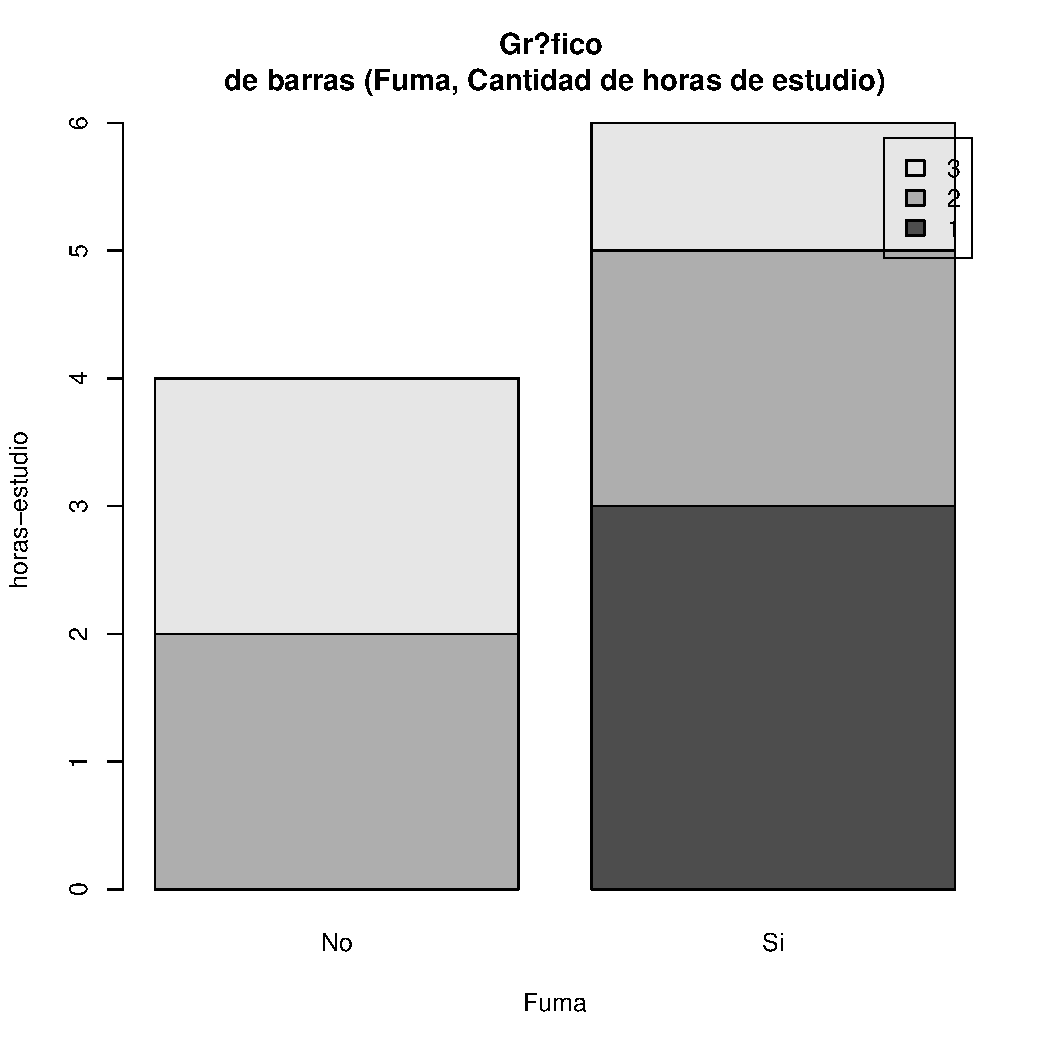
\includegraphics[width=\maxwidth]{figure/unnamed-chunk-3-1} 
\begin{kframe}\begin{alltt}
\hlcom{# Gr?fico de barras apiladas con la frecuencia de Fuma como altura }
\hlkwd{barplot}\hlstd{(}\hlkwd{table}\hlstd{(Estudia}\hlopt{$}\hlstd{Fuma, Estudia}\hlopt{$}\hlstd{Cantidad),} \hlkwc{beside} \hlstd{=} \hlnum{FALSE}\hlstd{,} \hlkwc{horizontal}\hlstd{=}\hlnum{FALSE}\hlstd{,}\hlkwc{main}\hlstd{=}\hlstr{"Gr?fico 
de barras (Cantidad de horas de estudio,Fuma)"}\hlstd{,} \hlkwc{legend.text} \hlstd{=T,} \hlkwc{xlab}\hlstd{=}\hlstr{"Cantidad de horas-estudio"}\hlstd{,}
\hlkwc{ylab}\hlstd{=}\hlstr{"Fuma"}\hlstd{)}
\end{alltt}


{\ttfamily\noindent\color{warningcolor}{\#\# Warning in plot.window(xlim, ylim, log = log, ...): "{}horizontal"{} is not a graphical parameter}}

{\ttfamily\noindent\color{warningcolor}{\#\# Warning in axis(if (horiz) 2 else 1, at = at.l, labels = names.arg, lty = axis.lty, : "{}horizontal"{} is not a graphical parameter}}

{\ttfamily\noindent\color{warningcolor}{\#\# Warning in title(main = main, sub = sub, xlab = xlab, ylab = ylab, ...): "{}horizontal"{} is not a graphical parameter}}

{\ttfamily\noindent\color{warningcolor}{\#\# Warning in axis(if (horiz) 1 else 2, cex.axis = cex.axis, ...): "{}horizontal"{} is not a graphical parameter}}\end{kframe}
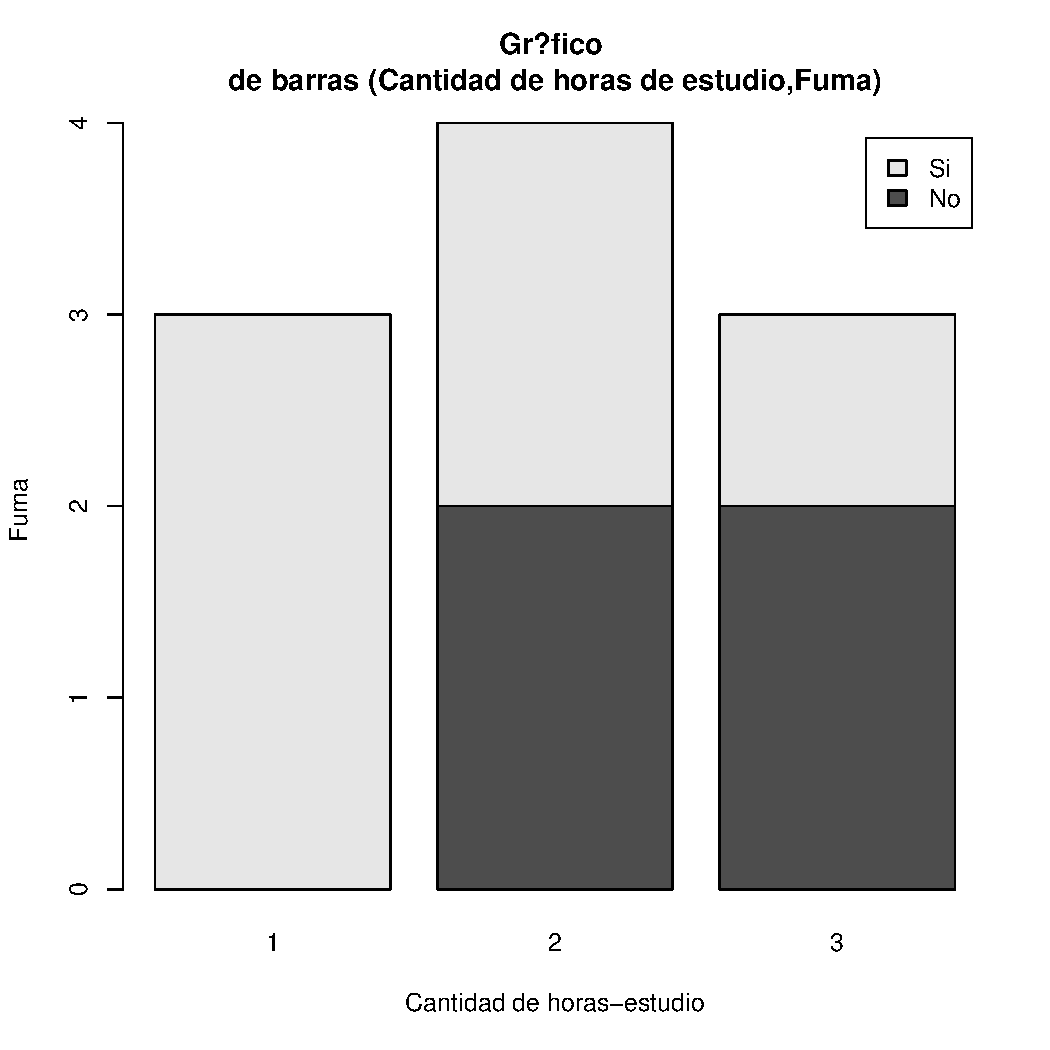
\includegraphics[width=\maxwidth]{figure/unnamed-chunk-3-2} 
\begin{kframe}\begin{alltt}
\hlcom{# Gr?fico de barras no apiladas y colocaci?n de leyenda }
\hlcom{# Crear un factor para los nombres en la leyenda }
\hlstd{Fuma}\hlkwb{=}\hlkwd{factor}\hlstd{(Estudia}\hlopt{$}\hlstd{Fuma); Fuma}
\end{alltt}
\begin{verbatim}
##  [1] Si No No Si No Si Si Si No Si
## Levels: No Si
\end{verbatim}
\begin{alltt}
\hlkwd{barplot}\hlstd{(}\hlkwd{table}\hlstd{(Estudia}\hlopt{$}\hlstd{Cantidad, Estudia}\hlopt{$}\hlstd{Fuma),} \hlkwc{main}\hlstd{=}\hlstr{"Gr?fico de barras (Fuma, Cantidad de horas 
de estudio)"}\hlstd{,} \hlkwc{xlab}\hlstd{=}\hlstr{"Fuma"}\hlstd{,} \hlkwc{ylab}\hlstd{=}\hlstr{"Cantidad dehoras-estudio"}\hlstd{,} \hlkwc{beside}\hlstd{=}\hlnum{TRUE}\hlstd{,} \hlkwc{legend.text}\hlstd{=T)}
\end{alltt}
\end{kframe}
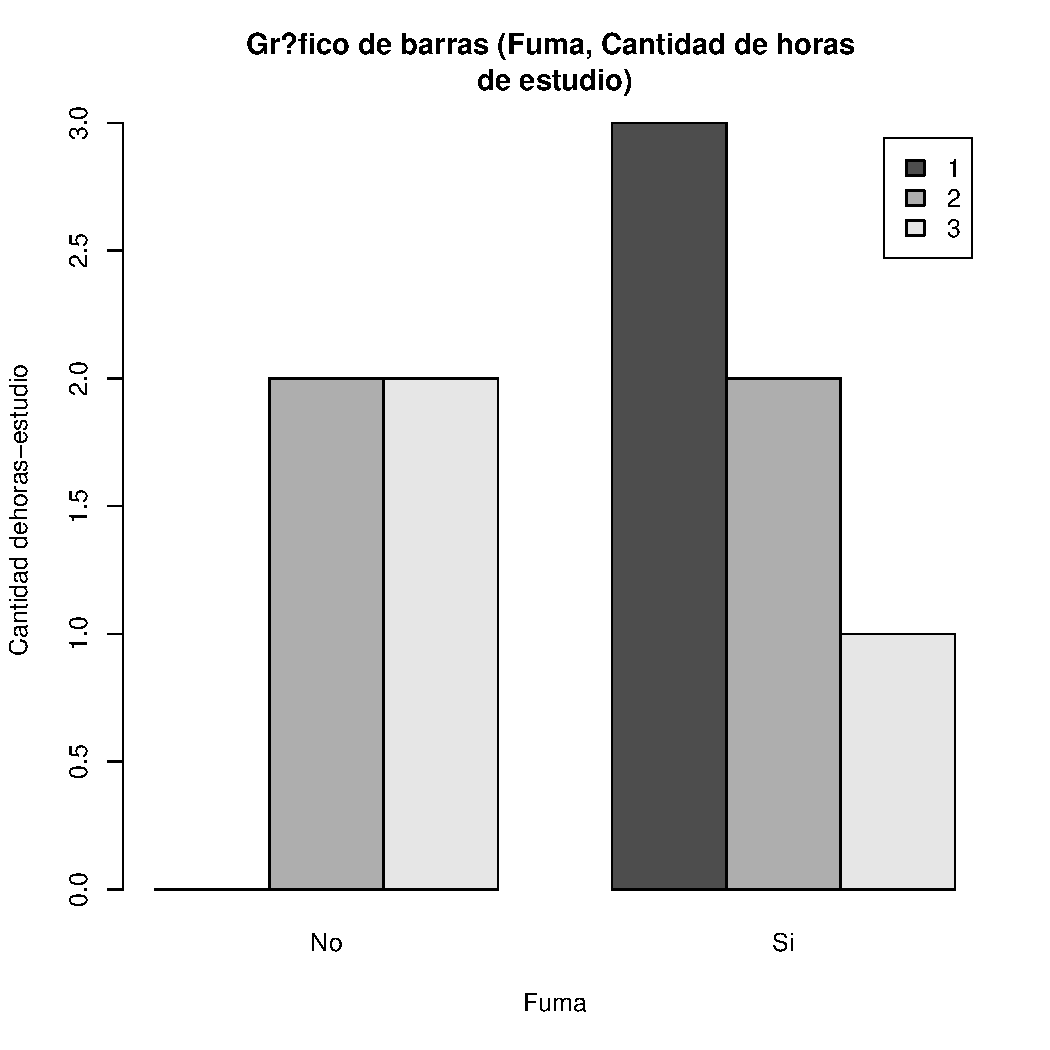
\includegraphics[width=\maxwidth]{figure/unnamed-chunk-3-3} 
\begin{kframe}\begin{alltt}
\hlkwd{barplot}\hlstd{(}\hlkwd{table}\hlstd{(Estudia}\hlopt{$}\hlstd{Cantidad, Estudia}\hlopt{$}\hlstd{Fuma),} \hlkwc{main}\hlstd{=}\hlstr{"Gr?fico de barras (Fuma, Cantidad de horas 
de estudio)"}\hlstd{,} \hlkwc{xlab}\hlstd{=}\hlstr{"Fuma"}\hlstd{,} \hlkwc{ylab}\hlstd{=}\hlstr{"Cantidad de horas-estudio"}\hlstd{,} \hlkwc{beside}\hlstd{=}\hlnum{TRUE}\hlstd{,}
\hlkwc{legend.text}\hlstd{=}\hlkwd{c}\hlstd{(}\hlstr{"menor que 5"}\hlstd{,} \hlstr{"5-10"}\hlstd{,} \hlstr{"mayor que 10"}\hlstd{))}
\end{alltt}
\end{kframe}
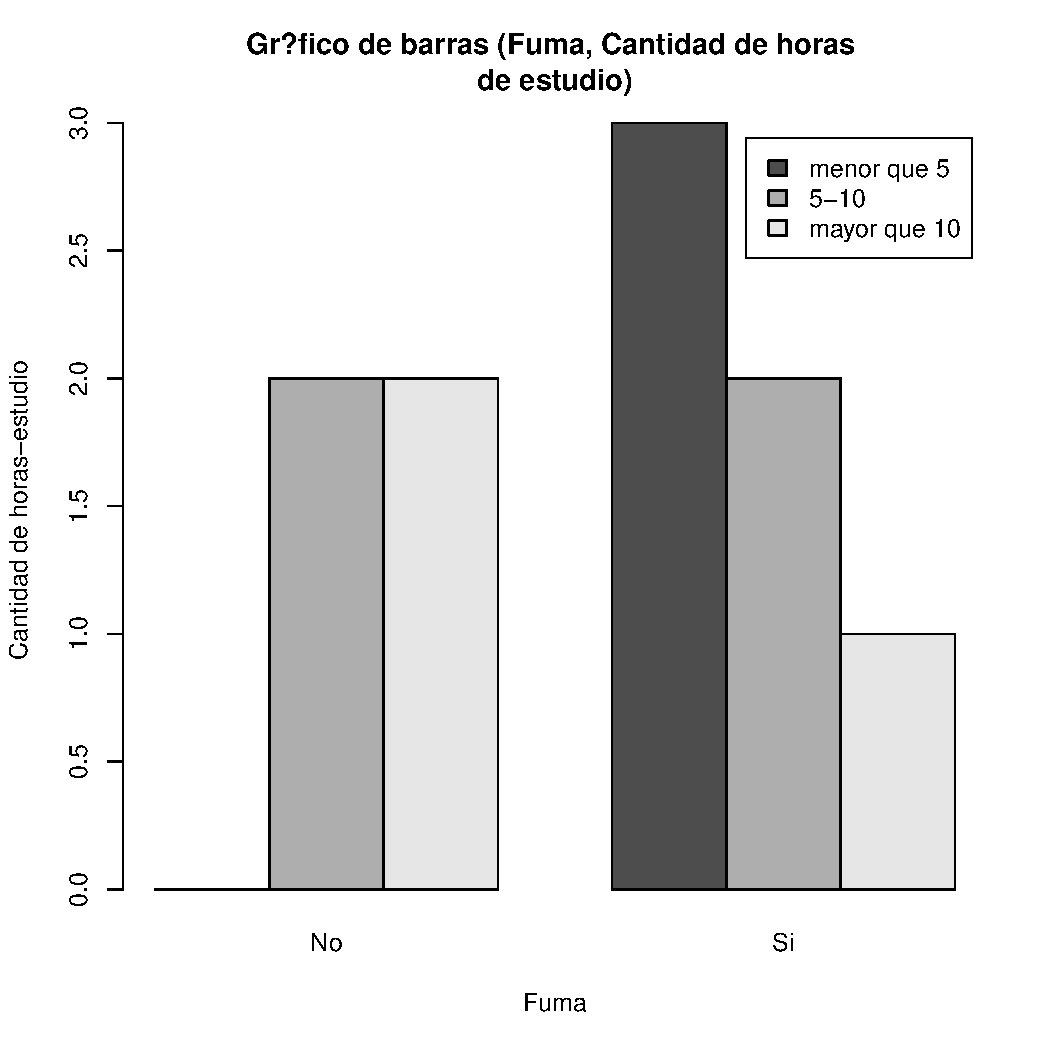
\includegraphics[width=\maxwidth]{figure/unnamed-chunk-3-4} 
\begin{kframe}\begin{alltt}
\hlcom{# Probabilidades esperadas para la prueba Chi-cuadrada }
\hlkwd{chisq.test}\hlstd{(tablaCont)} \hlopt{$}\hlstd{expected}
\end{alltt}


{\ttfamily\noindent\color{warningcolor}{\#\# Warning in chisq.test(tablaCont): Chi-squared approximation may be incorrect}}\begin{verbatim}
##     Cantidad
## Fuma   1   2   3
##   No 1.2 1.6 1.2
##   Si 1.8 2.4 1.8
\end{verbatim}
\end{kframe}
\end{knitrout}


\end{document}
